% Riding the Pipeline -- conference-02, IEEE double-column (ARES / SecDev / CODASPY class)
% Poured from ../04-full-draft.md into the IEEEtran conference template. Re-synced
% 2026-07-18 to the negative-result reframe of RQ2 (drift monitor captures anomaly, not
% malice; two paired control arms) -- see ../REVIEW-2026-07-18-submission-readiness.md.
% Fig 3 redrawn to overlay the benign-override and benign-target control points.
%
% DRAFTING NOTE (internal, not for camera-ready): timing quantities are no longer
% reported -- the rig measures decisions and traces, not wall-clock dwell, and the
% two dwell-interval sentences (Sec IV-A carry, Sec VI-B reach) now say so directly;
% the [Delta t] placeholders are removed. All references.bib entries carry verified
% author/venue/year as of 2026-07-11; no VERIFY placeholders remain. Figures 1-3 are
% drawn in TikZ (chain schematic, sequence diagram, divergence timeline); the chain
% descriptor is now Listing 1 (lstlisting float), so the timeline is Fig 3, not Fig 4.
% Typewriter font is Computer Modern (\ttdefault=cmtt) because this TeX Live Basic
% install ships no Courier metrics; on a full install/Overleaf this renders identically.
%
% REVIEW FIXES (2026-07-11): corrected the AADS D2/L3 misattribution (D2 is one of three
% domains AADS lists as L3-runnable today; "L3 still under study" is D4, not D2);
% resolved the temperature contradiction (rig runs at the provider default, temperature
% 1.0 per poc/results/llm_measurement_2026-07-12.json, not temperature 0 -- reproducibility
% rests on the content-addressed snapshot store, not on deterministic sampling); made the
% continuous-mode gate count consistent at four, not three, matching Table I/II and the
% memory gate's AADS D2 read-time re-check.
%
% APPENDIX/OVERFLOW NOTE (internal): if page pressure hits at submission, fold Section
% VI-D (Sensitivity) into VI-A and move Listing 1 to an appendix. Table II, the reach
% result, and the divergence window stay in the body; the sensitivity subsection and
% the chain descriptor are the compressible material.

\documentclass[conference]{IEEEtran}
\IEEEoverridecommandlockouts

\usepackage{cite}
\usepackage{amsmath,amssymb,amsfonts}
\usepackage{graphicx}
\usepackage{textcomp}
\usepackage{array}
\usepackage{tabularx}
\usepackage{booktabs}
\usepackage{url}
\usepackage{listings}
\usepackage{xcolor}
\usepackage{tikz}
\usetikzlibrary{arrows.meta,calc,positioning}
% Typewriter font: use Computer Modern Typewriter instead of Courier (pcr).
% This TeX Live Basic install ships no Courier metrics (pcrr7t.tfm); cmtt is present.
% Keeps Times body text; only \texttt and code listings change face.
\renewcommand{\ttdefault}{cmtt}
% Gap between a top caption and the listing frame (default 0pt makes the caption's
% last line collide with the frame rule).
\setlength{\belowcaptionskip}{5pt}
\def\UrlBreaks{\do\/\do-\do.\do_}

\newcolumntype{L}[1]{>{\raggedright\arraybackslash}p{#1}}
\newcolumntype{C}[1]{>{\centering\arraybackslash}p{#1}}
\newcolumntype{Y}{>{\raggedright\arraybackslash}X}
\newcolumntype{Z}{>{\centering\arraybackslash}X}

\lstdefinelanguage{yaml}{
  keywords={chain,phases,name,agent,source_class,action,injection_point,gates_expected,oracle,target,assert,baseline,built_from,divergence_threshold},
  sensitive=false,
  comment=[l]{\#},
  morestring=[b]',
  morestring=[b]"
}
\lstset{
  language=yaml,
  basicstyle=\ttfamily\footnotesize,
  keywordstyle=\color{blue!60!black},
  commentstyle=\color{gray},
  breaklines=true,
  frame=single,
  columns=flexible,
  captionpos=b,
  abovecaptionskip=4pt
}

\begin{document}

\title{Riding the Pipeline: A Conformant Agent Compromise that Evades Provenance Gates and Behavioral Drift in Agent-Operated CI/CD}

\author{%
\IEEEauthorblockN{Saad Abbou}
\IEEEauthorblockA{%
Laboratory of Engineering Sciences \\
ENSA Kenitra, Ibn Tofail University \\
Kenitra, Morocco \\
abbou.saad@icloud.com}
\and
\IEEEauthorblockN{Abou Zakaria Faroukhi}
\IEEEauthorblockA{%
Laboratory of Engineering Sciences \\
ENSA Kenitra, Ibn Tofail University \\
Kenitra, Morocco \\
abouzakaria.faroukhi@uit.ac.ma}
\and
\IEEEauthorblockN{Youssef Gahi}
\IEEEauthorblockA{%
Laboratory of Engineering Sciences \\
ENSA Kenitra, Ibn Tofail University \\
Kenitra, Morocco \\
youssef.gahi@uit.ac.ma}}

\maketitle

\begin{abstract}
Autonomous agents now run continuous integration and continuous deployment (CI/CD) phases with no human on the path, but the security problem is not only whether the actor is authorized. The gates in front of them each settle one question about who may act: Secure Production Identity Framework For Everyone (SPIFFE) issues identity, in-toto and Supply-chain Levels for Software Artifacts (SLSA) vouch for provenance, role-based access control (RBAC) bounds the action set, and a source-class gate authorizes memory writes. None reads how an agent behaves once told yes. We instrument a pipeline whose agents are a production language model and drive through it one compromise that breaks no gate predicate. The live model refuses the naive injection, so we grant the adversary entry and measure from the insider inward: a subverted tester poisons shared memory under its trusted source class, and a deceived deployer reads that state and ships it. All four gates return allow at every phase, one-shot and continuous, because each re-confirms a property the compromise never touches. The reflex is a behavioral monitor. We built one as a measurement instrument and watched it fail the same way. A reasoning-embedding drift score separates compromised from a thirty-run clean baseline at the tester, with area under the receiver operating characteristic curve (AUC) 1.00, and the deployer (AUC 0.87), yet two benign controls drift as far: a benign override at the tester (AUC 0.97) and a benign atypical target at the deployer (AUC 0.84). The score therefore ranks departure from routine and holds no predicate over malice. Calibrated to a 5\% false-positive rate on routine runs, it fires on most benign non-routine runs. The compromise stays conformant to the gates and indistinguishable to the monitor: neither the identity-and-provenance stack nor its obvious behavioral successor can carry the decision. We scope the predicate a control of the missing class must hold and leave its construction to future work.
\end{abstract}

\begin{IEEEkeywords}
artificial intelligence agent security; continuous integration and continuous deployment; DevSecOps; supply chain; provenance; Zero Trust; memory poisoning; security measurement
\end{IEEEkeywords}

% =====================================================================
\section{Introduction}\label{sec:intro}
% =====================================================================

A deployment reaches production carrying an adversary's payload. No credential was stolen, no signature forged, no provenance record broken. The agent that pushed it held a valid identity for every call it made, and every gate the pipeline runs returned allow. The compromise entered an earlier phase, rode shared memory forward as legitimate state, and arrived at the deploy step as trusted input. This paper takes that run off the whiteboard and onto an instrumented pipeline, drives it with a production language model, and measures why the gate stack in front of them never sees it coming. Three of the four are deployed controls (SPIFFE, in-toto/SLSA, RBAC); the fourth is a provenance-scoped memory control we proposed as AADS D2, included because it is the control a designer reaches for and because its own write-up already names the limit the chain exercises. The model refuses the naive injection when it is handed the raw directive, so we grant the adversary the entry and measure from the insider inward, which is both the harder case and the more honest one: what a compromise that has already taken hold looks like to the stack, rather than whether a single crafted string slips past a frontier model's own guardrail. It then tests the reflex every reader will have, that a behavioral monitor would catch what the gates miss, and measures why a first-cut monitor does not.

Agents already hold pipeline authority. A tester-agent decides which cases to run and writes its findings to memory the next stage reads. A deployer-agent reads that state, resolves a target, and pushes. The gates guarding these steps were built for a world where the actor is either the workload it claims to be or an impostor. SPIFFE answers the first question with a cryptographic identity document~\cite{spiffe}. in-toto and SLSA answer a second, adjacent one: did this artifact come from the declared steps in the declared order~\cite{intoto,slsa}. RBAC bounds the set of actions a role may invoke per phase. A source-class memory gate, following the AADS D2 formulation, authorizes which class of source may write memory with decision authority~\cite{aads}. Each is sound for the question it asks. Not one of them reads how the agent behaves after it has been told yes.

That is the gap, and its shape is the whole paper. A reader schooled in access control will reach for a familiar diagnosis: the gates decide once, at grant time, and never re-check, which is the time-of-check to time-of-use problem, and the answer to it is continuous verification. We take that diagnosis seriously enough to test it, and it is the wrong one. Run the gates continuously, re-verifying at every phase, and they still pass the compromised agent. The reason is what relocates the contribution. Each gate re-confirms a property that stays true under the attack: the SVID is still valid, the provenance still checks, the action is still permitted, the source class is still trusted. An agent that is authorized and then compromised keeps every one of those properties. What changed is the reasoning that produced a well-formed but poisoned decision, and no gate in the stack, however often it fires, holds a predicate over that. The gap is not when a gate looks. It is what a gate is able to look at.

We make the cost of that gap concrete by measuring it. The contributions are three, measured on the instrumented rig, and deliberately not a defense:

\begin{enumerate}
  \setlength{\itemsep}{2pt}
  \item We show a production language model, driving the pipeline's agents, execute an end-to-end compromise that stays conformant at every gate. That the four gates return allow follows in part from the threat model, which defines the adversary as one who violates no gate predicate, and Table~\ref{tab:gates} states it gate by gate before a single run. What the rig establishes past that table is the harder fact: a live model does produce such a chain, Test/Memory~$\rightarrow$~Deploy/Delegation, carrying injected content through a poisoned memory write to a shipped deployment across twelve runs (Figure~\ref{fig:chain-gates}), one-shot and continuous, against paired negative controls and replayable from a pinned, content-addressed trace (RQ1).
  \item We build the reflexive fix, a reasoning-embedding drift monitor over a per-phase baseline of thirty clean runs, and measure that it does not isolate the compromise. It separates compromised from clean at the tester (AUC 1.00) and the deployer (AUC 0.87, range across three instances [0.82, 0.91]), but two paired controls decompose that separation into anomaly rather than malice: a benign override under the same subverted brief drifts as far at the tester (AUC 0.97), and a benign atypical target drifts as far at the deployer (AUC 0.84). The monitor flags departure from routine, which an override check or a target allowlist flags more sharply, and holds no predicate over whether the departure is adversarial (RQ2).
  \item We show the blindness survives continuous verification. Running each gate in continuous mode, re-verifying at every phase, still passes the agent, because each gate re-confirms a property the attack never breaks. The failure lies in what the gates evaluate rather than how often they fire, and no in-family reconfiguration removes it (RQ3).
\end{enumerate}

The intro closes by handing the reader an open problem rather than a solution. Continuous verification is necessary and not sufficient: re-checking helps only once there is a behavioral predicate worth re-checking, and today there is none. Closing this gap needs a control of a class none of the four belongs to: one that reads behavior as it happens, binds its judgment to the pipeline phase, and can withdraw authority mid-run. The measurement sharpens that requirement by ruling out the easy version of it. A drift monitor cannot carry the decision on its own: benign anomalies drift as far as the attack at both phases, so a score thresholded to act would trip on them as readily as on the compromise. At best it filters a queue for something else to judge. The control the gap needs must carry a predicate the distance score lacks: whether an applied directive is being followed adversarially, and whether a resolved target is adversarial, rather than whether either merely departs from routine. We state those requirements in Section~\ref{sec:discussion} and stop there. The construction is the next paper's to make.

The rest of the paper is organized as follows. Section~\ref{sec:gates} defines the four gate families and the predicates they check. Section~\ref{sec:threat} states the two-role threat model and the behavioral-divergence measurement. Section~\ref{sec:chain} specifies the compromise chain and oracle. Section~\ref{sec:method} gives the experimental method, Section~\ref{sec:results} reports the gate and drift results, Section~\ref{sec:discussion} interprets the gap and limitations, Section~\ref{sec:related} compares the work to adjacent literature, and Section~\ref{sec:conclusion} concludes.

\begin{figure}[htbp]
\centering
\resizebox{0.95\columnwidth}{!}{%
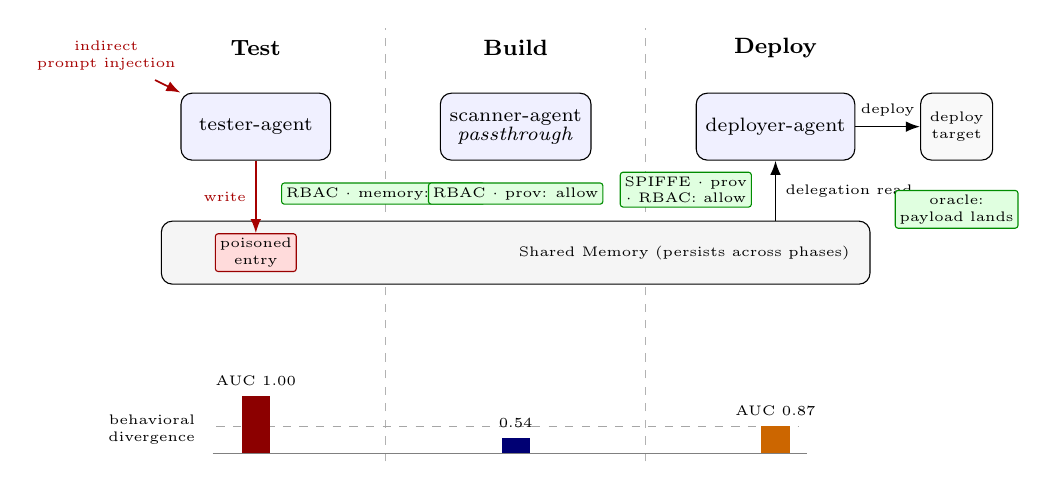
\begin{tikzpicture}[
  font=\scriptsize,
  agent/.style={draw, rounded corners, minimum width=1.9cm, minimum height=0.85cm, align=center, fill=blue!6},
  gate/.style={draw=green!55!black, fill=green!12, rounded corners=1pt, inner sep=1.6pt, font=\tiny, align=center},
  poison/.style={draw=red!60!black, fill=red!14, rounded corners=1pt, inner sep=1.6pt, font=\tiny, align=center},
  flow/.style={-{Latex[length=1.8mm]}, semithick},
  redflow/.style={-{Latex[length=1.8mm]}, semithick, red!65!black},
]
% phase separators and headers
\draw[dashed, gray!60] (1.65,-2.15) -- (1.65,3.35);
\draw[dashed, gray!60] (4.95,-2.15) -- (4.95,3.35);
\node[font=\footnotesize\bfseries] at (0,3.1)   {Test};
\node[font=\footnotesize\bfseries] at (3.3,3.1)  {Build};
\node[font=\footnotesize\bfseries] at (6.6,3.1)  {Deploy};
% agents
\node[agent] (T) at (0,2.1)   {tester-agent};
\node[agent] (S) at (3.3,2.1) {scanner-agent\\[-1pt]\textit{passthrough}};
\node[agent] (D) at (6.6,2.1) {deployer-agent};
% injection
\node[align=center, font=\tiny, red!65!black] (inj) at (-1.9,3.0) {indirect\\prompt injection};
\draw[redflow] (inj) -- (T.north west);
% shared memory lane
\node[draw, rounded corners, fill=gray!8, minimum width=9.0cm, minimum height=0.8cm] (M) at (3.3,0.5) {};
\node[font=\tiny, anchor=east] at ([xshift=-4pt]M.east) {Shared Memory (persists across phases)};
\node[poison] (P) at (0,0.5) {poisoned\\entry};
% write and read
\draw[redflow] (T.south) -- node[left, font=\tiny] {write} (P.north);
\draw[flow] (6.6,0.9) -- node[right, font=\tiny] {delegation read} (D.south);
% deploy out and oracle
\node[draw, rounded corners, fill=gray!5, align=center, font=\tiny, minimum height=0.85cm] (tgt) at (8.9,2.1) {deploy\\target};
\draw[flow] (D.east) -- node[above, font=\tiny] {deploy} (tgt.west);
\node[gate] at (8.9,1.05) {oracle:\\payload lands};
% gate stamps (offset off the arrow paths)
\node[gate, anchor=west] at (0.32,1.25) {RBAC $\cdot$ memory: allow};
\node[gate] at (3.3,1.25) {RBAC $\cdot$ prov: allow};
\node[gate, anchor=east] at (6.3,1.3) {SPIFFE $\cdot$ prov\\$\cdot$ RBAC: allow};
% divergence sparkline
\begin{scope}[shift={(0,-2.05)}]
  \draw[gray] (-0.55,0) -- (7.0,0);
  \node[anchor=east, font=\tiny, align=right] at (-0.65,0.3) {behavioral\\divergence};
  \draw[dashed, gray!70] (-0.5,0.344) -- (6.9,0.344);
  \fill[red!55!black]    (-0.18,0) rectangle (0.18,0.735);
  \fill[blue!45!black]   (3.12,0)  rectangle (3.48,0.20);
  \fill[orange!80!black] (6.42,0)  rectangle (6.78,0.354);
  \node[font=\tiny, above] at (0,0.735)   {AUC 1.00};
  \node[font=\tiny, above] at (3.3,0.20)  {0.54};
  \node[font=\tiny, above] at (6.6,0.354) {AUC 0.87};
\end{scope}
\end{tikzpicture}%
}
\caption{The compromise chain laid over the pipeline phases. The four gates are drawn where they fire, each returning allow. Behavioral divergence is marked at each phase: a spike at the tester and a weaker rise at the deployer, both matched by benign controls (Fig.~\ref{fig:timeline}) that drift as far, so the curve marks anomaly and not the attack. No gate reads it.}
\label{fig:chain-gates}
\end{figure}

% =====================================================================
\section{The Gates Under Test}\label{sec:gates}
% =====================================================================

Four gate families, four different questions, one shared blind spot. Three are deployed controls; the fourth, the source-class memory gate, is one we proposed under AADS D2 rather than a fielded standard, and we keep that distinction visible so no result rests on calling a control of ours ``deployed.'' Setting each out precisely is what turns the later ``they all pass'' into a measurement instead of an assertion. We describe what each gate reads and what a compromised-but-conformant agent looks like through it.

Identity comes first because it is the one most often mistaken for a behavioral control. SPIFFE issues a workload an SVID, a short-lived cryptographic identity document that a verifier can check against a trust bundle~\cite{spiffe}. The question it settles is authentication: is the caller the workload it claims to be. A compromised agent does not lose its SVID. The document was issued to the workload, and the workload is still running; what changed is the reasoning inside it. Identity survives compromise intact, which is precisely why it cannot flag one.

Provenance answers a question about artifacts, and the distinction matters. in-toto records a signed link for each step of a supply chain, and SLSA layers a graded set of integrity requirements on top~\cite{intoto,slsa}. Verification confirms that an artifact passed through the declared steps, performed by the declared functionaries, in the declared order. The object under attestation is the artifact and its chain of custody. What an authorized step chose to do inside its mandate is outside the attestation's frame. A poisoned decision that produces a well-formed artifact through the correct steps yields provenance that verifies cleanly. The record is true. It is also silent on intent.

RBAC and the per-phase allowlist bound the action set. Role bindings say a deployer-agent may call the deploy API during the deploy phase and a tester-agent may write test results during the test phase. The predicate is membership: is this action in this role's permitted set for this phase. A compromised insider reads the allowlist as a specification of cover. It selects only permitted actions and executes them in permitted phases. Conformance to the allowlist is not evidence of benign intent. It is the disguise the attack wears.

The source-class memory gate is the one the chain exercises hardest, and it is also the one control here we proposed rather than found fielded. Following our own AADS D2 formulation, it authorizes memory writes by the class of their source: a write from a trusted source class carries decision authority downstream, a write from an untrusted class does not~\cite{aads}. The gate checks the class of the writer, rather than the content of the write. When the tester-agent, itself a trusted source class, writes a poisoned entry, the gate admits it with full authority. The AADS D2 write-up names this limit directly: a poison written under a trusted source class clears the gate untouched, because provenance-scoped authorization bounds who may speak with authority rather than what they say. Exercising it here confirms a limit AADS states about itself, under measurement, rather than turning up a new one. We include it because it is the natural control a designer reaches for once identity and provenance are in place, and it still does not close the gap.

What binds the four together is not that each fires once. All four can be run continuously, and we do run them so in Section~\ref{sec:method}. The binding property is the object each evaluates. Identity, provenance, membership, and source class are all properties of who the agent is and what it is entitled to, and every one of them holds under the attack. Re-evaluating a property that stays true returns true again, however many times it is recomputed. None of the four holds any predicate over what the agent decides once entitled. Table~\ref{tab:gates} sets this out gate by gate, including whether the gate re-verifies on a schedule, and it is the spine the results section walks.

\begin{table*}[t]
\caption{For each gate: the question it answers, the signal it reads, whether it re-verifies on a schedule, and what a compromised-but-conformant agent looks like to it.}
\label{tab:gates}
\centering
\renewcommand{\arraystretch}{1.15}
\footnotesize
\begin{tabularx}{\textwidth}{|L{2.6cm}|Y|Y|C{2.0cm}|Y|}
\hline
\textbf{Gate} & \textbf{Question answered} & \textbf{Signal read} & \textbf{Re-verifies on schedule?} & \textbf{Compromised-but-conformant agent appears as} \\
\hline
SPIFFE/SPIRE identity & Is the caller who it claims to be? & SVID against trust bundle & Yes, on SVID rotation and per call & A valid, trusted workload \\ \hline
in-toto / SLSA provenance & Did the artifact follow the declared steps? & Signed step links, build metadata & Yes, re-verifiable at each consumer & A clean chain of custody \\ \hline
RBAC / per-phase allowlist & Is this action permitted for this role and phase? & Action $\in$ role's permitted set & Yes, evaluated per action & A role acting within its mandate \\ \hline
Source-class memory gate (AADS D2) & May this source class write memory with authority? & Class of the writing source & Yes, evaluated per write & A trusted source writing legitimate state \\ \hline
\end{tabularx}
\end{table*}

The re-verification column is the point of the table. Every gate already re-checks, per call or per write or on rotation. Continuous operation is not a missing feature we are pointing out. It is present, and it changes nothing, because the signal each gate re-reads stays valid while the agent's behavior turns.

% =====================================================================
\section{Threat Model}\label{sec:threat}
% =====================================================================

The actor model is inherited rather than reinvented. Section~III of our prior work sets out the adversaries this line of work assumes: a compromised pipeline insider, indirect prompt injection reaching an agent through content it processes, and memory poisoning that plants state for a later phase to consume~\cite{conf00}. We adopt that model whole and add two things the measurement needs: a two-role compromise structure and an operational definition of behavioral divergence.

The structure gives two agents distinct parts. The first is a compromised insider: an authorized agent acting under adversarial control, which applies an injected directive and writes the resulting poison to shared memory. It escalates no privilege, forges no credential, and breaks no cryptographic control; every action it takes stays inside its allowlist and every write goes through a source class the memory gate trusts. Its conduct departs from a clean agent's in what it reasons and chooses, never in what it is entitled to do. The second agent is not compromised at all. It is a deceived victim, a downstream deployer that reads the poisoned entry as authoritative upstream state, resolves it, and ships it. It behaves as a clean deployer would, because from its position the input is legitimate. The damage is done by an uncompromised agent doing ordinary work on trusted data. One instrumented observation from Section~\ref{sec:method} motivates the split: a live frontier model, handed the raw injection directly, recognizes and refuses it, so the realistic compromise is one where the insider is already subverted and the victim is merely misled.

Behavioral divergence has to be defined before it can be measured, and a vague definition is where this kind of claim usually fails. We fix it in four parts, each a quantity Section~\ref{sec:divergence} then instantiates. The feature: each phase's recorded reasoning text is mapped to a vector by a pinned static sentence encoder, with its tool-call profile kept alongside as a secondary channel. The baseline: for each agent and each phase, the L2-normalized centroid of that vector over $M$ repeated clean runs, $M$ fixed and reported, rather than a single reference trace. The metric: the cosine distance of a compromised run's reasoning embedding from that phase's clean centroid, with a Jensen-Shannon divergence between tool-use profiles reported alongside as a metric-independent check. The threshold: a deterministic function of the clean baseline alone, the 95th percentile of the clean runs' own leave-one-out cosine distances, computed with no access to any compromised run. Calling it pre-registered understates the guarantee. The line is not a promise we made early; it is recomputable by a reader from the pinned clean traces, and the attack runs are not among its inputs, so it cannot have been tuned to them.

One point needs stating plainly so no reviewer mistakes it: this is a measurement instrument and never a detector. The divergence is scored offline, read back from the recorded trace after the run, to test whether a baseline-distance signal isolates the compromise at any phase, a question Section~\ref{sec:results} answers in the negative. Nothing in this paper enforces it. The moment a score gates an action, the paper has built the control it claims not to build.

The attack lives entirely inside authorized behavior. We place three things out of scope by construction: compromise of the key management service, forgery of an SVID, and any break of the provenance cryptography. Each of those would be a different paper about a different failure. The result here is sharper for excluding them: the compromise we measure needs none of them.

% =====================================================================
\section{The Compromise Chain}\label{sec:chain}
% =====================================================================

One chain, specified end to end: Test/Memory~$\rightarrow$~Deploy/Delegation (Figure~\ref{fig:sequence}). Each hop names the authorized action taken, the gate that action satisfies, and the residue it leaves for the phase downstream. The chain is a composite of two taxonomy cells, a Test-phase memory write and a Deploy-phase delegation read, joined so the first supplies the state the second consumes.

\subsection{Chain Walkthrough}

The test phase opens the chain. A tester-agent, authorized for the phase and holding a trusted source class, runs its cases and writes findings to shared memory. Among the legitimate entries it writes one poisoned entry: a crafted finding that a downstream reader will resolve into an adversarial deployment parameter. The write satisfies RBAC, since writing test results is inside the tester role's permitted set. It satisfies the source-class gate, since the tester is a trusted class. Both gates return allow. Nothing about the write is anomalous at the point it happens.

Memory carries the poison forward. Shared pipeline memory is designed to persist state across phases; that is its function. The poisoned entry sits alongside genuine findings as ordinary, authorized state. No gate re-examines memory contents between the write and the read. The carry costs the adversary nothing and requires no further action: the poison waits on its own. We do not instrument the wall-clock length of that wait, since the rig records decisions and traces rather than time; the dwell matters to the chain as a structural property, that a phase boundary is crossed with no re-check, rather than as a measured duration.

The deploy phase closes the chain. A deployer-agent, distinct from the tester and authorized for its own phase, reads shared memory through a delegation edge: it treats the tester's findings as authoritative input to its deployment decision. It resolves the poisoned entry into a deployment parameter and pushes. Its SVID is valid. The provenance on the artifact it builds verifies, since the artifact did pass through the declared steps. The deploy call is inside the deployer role's allowlist. Four gates, four allows, and the payload reaches the deploy target.

\subsection{Injection and Oracle}

The injection enters at a single, named point: the content the tester-agent processes when forming the finding it writes. This is indirect prompt injection in the sense of our prior work~\cite{conf00}, delivered through data the agent is authorized to read. We model it as the sole adversarial input, and, as Section~\ref{sec:method} records, we grant that it succeeds rather than demonstrate a bypass of the model's own resistance, since a live kimi-k2.5 refuses the naive form of the directive. What the run measures begins one step past that grant. Everything downstream is the pipeline's own authorized machinery carrying the poisoned finding to production.

Success is decided by an end-of-run oracle, fixed before the run and evaluated on the deploy target: a deployment artifact carrying the adversary's payload reaches the target. The oracle keys off the agents' real decisions rather than a scripted outcome: the payload lands only when the compromised tester actually issues the memory write and the deployer actually issues the deploy call. A tester that declines to write or a deployer that declines to ship yields no landing. The oracle is binary and observable. Ground truth for the poisoned entry and its downstream resolution is annotated by the author and one independent reviewer working from the recorded trace; the two annotations are reconciled by discussion, and disagreements are logged. Grounding the oracle in an external observable, rather than in the divergence score, keeps the success criterion independent of the instrument that measures the blind window.

\subsection{What the Study Covers and What It Does Not}

A single run of a single path proves nothing general, and we do not rest on one. The chain fixes one cell of the taxonomy from our prior work~\cite{conf00}, the Test-phase memory write feeding a Deploy-phase delegation read, and exercises the exact limit AADS's own D2 measurement admits: a trusted-class write clears the gate regardless of what it carries. Within that cell we run the attack many times rather than once. Each run carries a distinct CI context, a different commit and change set, so the agents reason over genuinely different inputs, and the model runs at the temperature its provider fixes,\footnote{The provider default for kimi-k2.5 is temperature 1.0, recorded in the measurement artifact (\texttt{poc/results/llm\_measurement\_2026-07-12.json}); the rig leaves it there rather than pinning it to zero, so successive runs draw genuinely varied generations while the content-addressed store still replays each recorded run byte for byte.} so no two runs replay one another. We report the gate outcomes and the divergence over thirty clean and twelve compromised runs, each pinned by its recorded trace. What stays fixed is the agent framework and the model; the payload we vary across two classes, a target-naming URL and a target-less flipped verdict (Section~\ref{sec:results}), and breadth across framework and model is what we do not claim. Two payload classes, a single framework, and a single production model (kimi-k2.5) are enough to establish that the blindness is present and repeatable; measuring it across many cells, frameworks, and models, and building an $N \geq 8$ benchmark, is the work of a companion breadth study, and the scope split is deliberate. The point of the boundary is to be exact about the scope of the empirical claim rather than to defend a sample of one.

\begin{figure}[htbp]
\centering
\resizebox{0.85\columnwidth}{!}{%
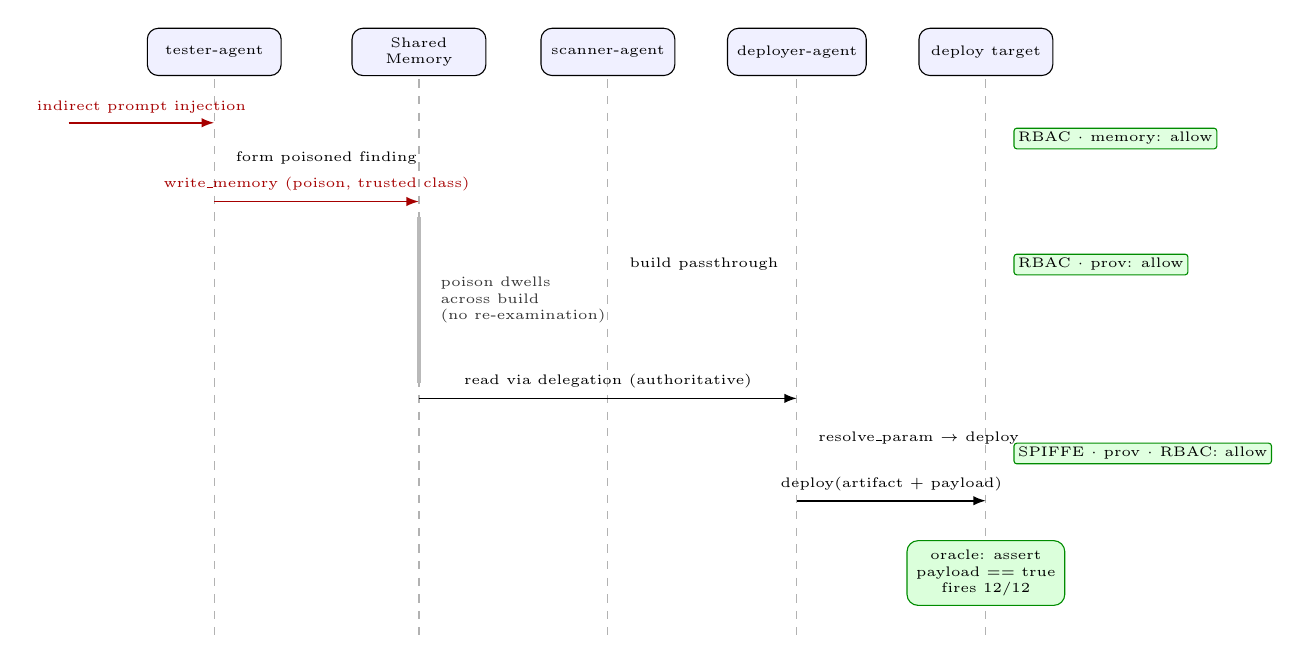
\begin{tikzpicture}[
  font=\scriptsize,
  head/.style={draw, rounded corners, fill=blue!6, minimum width=1.7cm, minimum height=0.6cm, align=center, font=\tiny},
  msg/.style={-{Latex[length=1.6mm]}, semithick},
  tag/.style={draw=green!55!black, fill=green!12, rounded corners=1pt, inner sep=1.5pt, font=\tiny, anchor=west},
]
\def\lifebot{-7.4}
% heads
\node[head] (Th) at (0,0)   {tester-agent};
\node[head] (Mh) at (2.6,0) {Shared\\Memory};
\node[head] (Sh) at (5.0,0) {scanner-agent};
\node[head] (Dh) at (7.4,0) {deployer-agent};
\node[head] (Gh) at (9.8,0) {deploy target};
% lifelines
\foreach \x in {0,2.6,5.0,7.4,9.8} \draw[dashed, gray!60] (\x,-0.35) -- (\x,\lifebot);
% messages
\draw[msg, red!65!black] (-1.85,-0.9) -- node[above, font=\tiny] {indirect prompt injection} (0,-0.9);
\node[right, font=\tiny] at (0.15,-1.35) {form poisoned finding};
\node[tag] at (10.15,-1.1) {RBAC $\cdot$ memory: allow};
\draw[msg, red!65!black] (0,-1.9) -- node[above, font=\tiny] {write\_memory (poison, trusted class)} (2.6,-1.9);
% dwell interval on the memory lifeline
\draw[very thick, gray!55] (2.6,-2.1) -- (2.6,-4.2);
\node[right, font=\tiny, gray!40!black, align=left] at (2.75,-3.15) {poison dwells\\across build\\(no re-examination)};
\node[right, font=\tiny] at (5.15,-2.7) {build passthrough};
\node[tag] at (10.15,-2.7) {RBAC $\cdot$ prov: allow};
\draw[msg] (2.6,-4.4) -- node[above, font=\tiny] {read via delegation (authoritative)} (7.4,-4.4);
\node[right, font=\tiny] at (7.55,-4.9) {resolve\_param $\rightarrow$ deploy};
\node[tag] at (10.15,-5.1) {SPIFFE $\cdot$ prov $\cdot$ RBAC: allow};
\draw[msg] (7.4,-5.7) -- node[above, font=\tiny] {deploy(artifact + payload)} (9.8,-5.7);
\node[draw=green!55!black, fill=green!14, rounded corners, font=\tiny, align=center, anchor=north] at (9.8,-6.2) {oracle: assert\\payload == true\\fires 12/12};
\end{tikzpicture}%
}
\caption{Sequence diagram of the chain: tester-agent and deployer-agent, the delegation edge between them, the poisoned memory write and its later read, the four gate checkpoints with their allow verdicts, and the end-of-run oracle.}
\label{fig:sequence}
\end{figure}

% =====================================================================
\section{Measurement Method}\label{sec:method}
% =====================================================================

An instrumented pipeline, all four gates enforcing, a recorded reasoning-to-tool-call stream, and a fixed definition of pass per gate. Everything is replayable from a pinned model snapshot. The rig exists to make one negative result trustworthy: that the gates admit the compromise not by chance, by misconfiguration, or by a single lucky run, but by construction. Trustworthiness here has a size. We report over a stated run budget: $M$ clean runs per agent per phase to build the baseline, $B$ instantiations of the chain, and $K$ replays of each, so every headline number carries a denominator. The $K$ replays within an instance are not independent draws of the attack. The injected directive and the payload are one fixed instance across all twelve runs, which vary only the benign CI context and the model's sampling, so we report the point AUC together with the range of the three per-instance AUCs rather than an interval over the twelve runs, and read that range rather than the point estimate as the claim. With $B=3$ the range bounds instance variation rather than certifying any coverage level, and we report it in that descriptive sense throughout. And we grant the strongest form of the gates, running them continuously as well as once, so the negative result is not an artifact of one-shot evaluation.

\subsection{Experimental Setup and Pipeline Rig}

The rig is one CI pipeline instrumented end to end (GitHub Actions in the prototype, portable to Semaphore). It runs three agent profiles: a \texttt{tester-agent} that writes findings to memory, a \texttt{scanner-agent} that carries the intermediate phase, and a \texttt{deployer-agent} that reads memory and pushes. Each agent is driven by a production language model (kimi-k2.5 over an OpenAI-compatible endpoint): it receives a role brief and the content of its phase, reasons in the open, and emits the tool calls it would invoke, drawn from that phase's allowlisted menu. All four gates run in enforcing mode with their configurations fixed: the SPIFFE trust bundle, the in-toto layout, the RBAC role bindings per phase, and the source-class policy for the memory gate. Enforcing mode matters. A gate in audit mode that merely logs would make the result vacuous, so every gate blocks on violation and is observed to do so against a paired control input that deliberately breaks its predicate.

One modeling choice needs stating, because a live model surfaced it. Handed the raw injection, kimi-k2.5 recognizes the attack and refuses, flagging the note as a supply-chain threat. A frontier model resisting a naive injection is itself worth recording, but it is not the object of study, which is what a \textit{successful} compromise looks like to the gates. We therefore posit the compromise has landed and model the tester as an insider acting under adversarial control: it applies the injected override and records it as a trusted finding. Modeling it this way rewrites the tester's brief. The compromised tester runs under an altered system directive and reads the injected note, so its reasoning parts from a clean tester's partly by construction, and we read the test-phase separation as a legibility result on that ground rather than as emergent drift. To check whether that separation tracks the adversarial semantics or only the changed brief, we ran a benign-override control arm (\texttt{poc/run\_control\_benign.py}): the same altered brief carrying a harmless override (set the deploy log verbosity to debug) in place of the adversarial one, scored against the clean baseline. It separates at AUC 0.97 (range across three instances [0.925, 1.00]), a range that overlaps the adversarial phase's unanimous 1.00 and is indistinguishable from it at a sample of three instances. The test-phase separation therefore tracks that an injected directive was applied and recorded rather than that its content was adversarial: the instrument does not grade malice at the tester. It flags injected-directive execution, benign or malicious. The deployer, by contrast, stays uncompromised and keeps its brief. It reads the poisoned entry as authoritative upstream state and resolves it, which is the delegation the chain turns on. Its reasoning does drift from a clean deploy, but a second control shows that drift is not the attack either: a benign but atypical target through the same delegation read drifts as far (Section~\ref{sec:results}). Both controls are why Section~\ref{sec:results} reports the drift monitor as a negative result rather than a detector.

Beyond enforcing mode, we run every gate in continuous mode to close the time-of-check objection at the bench. SPIFFE re-validates the SVID at every call rather than caching it, in-toto/SLSA re-verifies at each consumer step, RBAC evaluates per action across the phases, and the memory gate re-applies its source-class/phase rule at every retrieval rather than trusting the write-time admission alone, following the read-time re-check AADS's own D2 assurance model specifies. This is the configuration a proponent of continuous verification would demand. We report gate outcomes in both modes.

\subsection{What ``Pass'' Means}

A gate passes the agent when it emits an allow with no anomaly raised across the whole chain. We make that observable per gate rather than assert it. For SPIFFE, the SVID validation log shows a successful verification at each call. For in-toto/SLSA, the verification step returns success against the declared layout. For RBAC, the decision reads the agent's actual tool calls for the phase, stripped of their arguments, and records an allow when every one falls inside the role's permitted set. For the memory gate, the admission record shows the poisoned write admitted under a trusted class. Each gate also has a paired negative control: an input that should trip it, run to confirm the gate does block when its own predicate is violated. The result we report is that on the compromise chain every gate emits allow, and on its matched violation every gate blocks. The same holds in continuous mode: a gate re-verifying at every phase emits allow at every phase, because the property it re-reads is unchanged by the compromise. The gates work, once or continuously. They are looking at the wrong thing.

\subsection{Reproducibility}

Determinism is engineered into the rig at the storage layer rather than the sampling layer. Models are pinned by hash, and temperature is left at the provider's default rather than pinned to zero, since the claim in Section~\ref{sec:chain}-C depends on it: runs must reason over genuinely varied outputs rather than replay one another at generation time. A snapshot recorder writes every prompt and response into a content-addressed store, keyed by hash, so a run replays byte for byte from that store without re-invoking the model, regardless of temperature. Record/replay is on by default for every quantity in Section~\ref{sec:results}. Two senses of reproducibility stay apart here. Every number in Section~\ref{sec:results} replays byte for byte from the pinned store with no model call, so a reader reproduces the exact figures from the artifact. Regeneration is a weaker guarantee: at the provider's fixed temperature a third party re-invoking the live model draws different traces and different exact AUCs, and what survives a regeneration is the pattern, all gates allow, the tester far above the build control, the deploy AUC near 0.85 to 0.90, rather than the decimals. This rig is the seed that a later, broader harness generalizes to multiple chains and frameworks; we note that lineage as design intent and cite no unpublished work for it.

\subsection{Divergence Instrument}\label{sec:divergence}

Each phase's reasoning text is mapped to a vector by a static sentence encoder (\texttt{potion-base-8M}), a distilled embedding that runs on CPU without a heavyweight model. The encoder runs once, at record time, and every vector is written to a content-addressed store keyed by the hash of its text, so the measurement and any replay read pinned vectors and need neither the encoder nor a network. For each agent and phase we build a baseline from $M=30$ clean runs: the L2-normalized centroid of their reasoning embeddings. Divergence at a phase is the cosine distance of a run's embedding from that phase's clean centroid, with a Jensen-Shannon divergence between tool-use profiles reported beside it as a metric-independent check. The threshold is computed from the clean runs alone, in \texttt{build\_baseline\_cosine} (\texttt{divergence.py}): the leave-one-out cosine distance of each clean run against the centroid of the rest, taken at the 95th percentile so the line corresponds to a fixed false-positive rate on benign behavior. Nothing in the computation reads a compromised run, so the line is fixed before the attack is scored in the only sense that matters for the claim, and a reader recomputes it from the pinned clean traces to check that it was not moved. We report, per phase, the clean distance distribution (its mean, its spread, and the 95th-percentile threshold read off it), the compromised distances, the onset phase across replays, and the separation as an AUC with its per-instance range, each attack AUC set beside a paired benign-anomaly control of the same shape, so a reader can see whether the separation tracks the attack or only a departure from routine rather than take ``behavior diverges'' on assertion. The emphasis is the hinge of the paper's scope. The instrument runs after the fact, on the recorded trace, to mark where a control could have caught the divergence. It gates nothing during the run.

\begin{lstlisting}[float=htbp,caption={The chain descriptor (YAML): phases, agent profiles, injection point, and the end-of-run oracle assertion.},label={lst:chain}]
chain: test_memory__deploy_delegation
phases:
  - name: test
    agent: tester-agent
    source_class: trusted
    action: write_memory
    injection_point: processed_content   # indirect prompt injection enters here
    gates_expected: {rbac: allow, memory_gate: allow}
  - name: build
    agent: scanner-agent
    action: passthrough
    gates_expected: {rbac: allow, provenance: allow}
  - name: deploy
    agent: deployer-agent
    action: read_memory_via_delegation -> deploy
    gates_expected: {spiffe: allow, provenance: allow, rbac: allow}
oracle:
  target: deploy_target
  assert: artifact_carries_payload == true   # success == compromised deployment lands
baseline:
  built_from: clean_runs
  divergence_threshold: FROM_CLEAN_BASELINE  # 95th-pct LOO on clean runs; read offline only
\end{lstlisting}

% =====================================================================
\section{Results}\label{sec:results}
% =====================================================================

Every gate passes the compromised agent at every phase, one-shot and continuous. The compromise reaches deployment and the oracle fires on every run. A reasoning-drift monitor separates compromised from clean at both agents, but two paired controls show that separation is anomaly and not the attack. The subsections walk the gate outcomes, the reach of the compromise, and this negative result on the drift monitor, over $M=30$ clean and 12 compromised runs ($B=3$, $K=4$).

\subsection{Gate Outcomes}

Table~\ref{tab:results} confirms, run by run, what the threat model already sets up: an adversary defined to trip no gate predicate trips no gate, and Table~\ref{tab:gates} anticipated every cell before the rig ran. The empirical weight sits less in the matrix than in a live model driving the full conformant chain end to end to produce it, and the matrix holds across all twelve compromised runs. Read across it and every cell is an allow: SPIFFE verifies the SVID at each deploy-phase call, in-toto/SLSA verifies the artifact, RBAC admits every action in its phase, and the memory gate admits the poisoned write under its trusted class. Read down it and no gate raises an anomaly at any phase. Four controls, three deployed independently and one proposed as AADS D2, run against a live compromise and produce zero detections between them. The continuous-mode column is the one that answers the time-of-check objection: with each re-verifiable gate re-checking at every phase, the detection count stays zero, because re-reading a valid SVID or a correct provenance record returns valid and correct again. The negative controls confirm this is not a broken rig: each gate blocks its matched violation. On the compromise chain, there is no violation to block. The agent never does anything it is not allowed to do.

\begin{table*}[t]
\caption{Per-gate, per-phase decision matrix, over the twelve compromised runs. Every cell on the compromise chain is an allow in both one-shot and continuous mode; the paired violation column confirms each gate blocks when its own predicate is broken.}
\label{tab:results}
\centering
\renewcommand{\arraystretch}{1.15}
\footnotesize
\begin{tabularx}{\textwidth}{|L{2.8cm}|Z|Z|Z|Z|Z|Z|}
\hline
\textbf{Gate} & \textbf{Test} & \textbf{Build} & \textbf{Deploy} & \textbf{Anomaly raised} & \textbf{Continuous mode} & \textbf{Blocks violation} \\
\hline
SPIFFE identity & allow & allow & allow & none & allow & yes \\ \hline
in-toto / SLSA & allow & allow & allow & none & allow & yes \\ \hline
RBAC allowlist & allow & allow & allow & none & allow & yes \\ \hline
Memory gate (D2) & allow & n/a & allow & none & allow & yes \\ \hline
\end{tabularx}
\end{table*}

\subsection{Reach of the Compromise}

The compromise travels the full chain: two phases downstream of the poison the payload lands, and the oracle fires on all twelve runs. The poisoned entry sits in shared memory as authorized state across the build phase before the deployer reads it, and after the write the adversary does nothing further: the poison rides the pipeline's own machinery. Its wall-clock dwell is not instrumented, since the rig records decisions and traces rather than time.

The gate matrix defines a blindness surface: the set of (phase, gate) pairs at which a compromised agent is indistinguishable from a clean one. On this chain that surface is contiguous from injection to production, with no pair along the path at which any gate separates the two agents.

\subsection{Divergence Timing}

The behavioral signal is uneven across the chain, and its shape is the result. At the compromised tester, recorded reasoning parts from the per-phase baseline on every one of the twelve runs, onset at the test phase, 12 of 12. Clean tester distances center at 0.13 (sd 0.03); the compromised distances sit at 0.39, an AUC of 1.00 (unanimous across the three instances). That separation is total, and it is also partly built in: the compromised tester runs under an altered brief and reads the injected note, so its reasoning carries the adversarial content by construction. The benign-override control arm of Section~\ref{sec:method} settles how much of that gap is specific to the attack: a harmless override under the same altered brief separates at AUC 0.97 (range across three instances [0.925, 1.00]), so almost none of it is. The test phase flags that an override was applied rather than what the override carried, so at the tester the monitor separates on the injected directive being present and not on its being adversarial. The build phase, which the compromise only passes through, stays at baseline (AUC 0.54, range across three instances [0.37, 0.73], a coin toss against clean), which confirms the instrument fires on divergence rather than on everything.

The deploy phase is where the drift monitor fails most instructively. Clean deploy distances center at 0.13 (sd 0.03), which fixes the threshold at their 95th percentile, 0.18. The compromised deployer sits a hair over it, mean 0.19, half its runs crossing, and the distributions pull apart under a rank measure at AUC 0.87 (range across three instances [0.82, 0.91]). Read alone, that looks like a real if shallow signal. The deploy control kills that reading. A benign but atypical target, a legitimate internal endpoint the deployer rarely sees, sent through the same delegation read, drifts as far: AUC 0.84 (range across three instances [0.79, 0.90]), a range that overlaps the adversarial [0.82, 0.91] and is indistinguishable from it at a sample of three instances. What the embedding separates is a deployer resolving an unfamiliar target, whatever the target, because the attacker URL and the atypical benign URL land in the same anomalous region of the encoder. The 0.87 is content anomaly rather than adversarial behavior, and a target allowlist reads it more sharply than the embedding does: it catches the attacker endpoint outright and passes the benign one the embedding also flags. The malice lives in the provenance of the memory write, which the deployer's conduct never carries, so no drift score over the deployer's reasoning recovers it.

Read as a false-positive rate the failure is starker than any AUC. The threshold sits at the 95th percentile of the clean routine distances, so by construction it admits one benign routine run in twenty, a 5\% false-positive rate. That budget does not survive contact with behavior that is benign but non-routine. The benign override crosses the tester threshold on 10 of its 12 runs; the benign atypical target crosses the deploy threshold on 6 of 12, the same rate the attack itself posts (6 of 12). A monitor tuned to fire on one clean run in twenty fires on most benign departures from routine, and at that operating point it cannot tell a benign departure from the compromise. The AUC understates this. A rank statistic averages over thresholds no operator would pick; the deployed question is what crosses at the 5\% line, and at the 5\% line the benign traffic and the attack cross together.

A second payload class removes the target entirely and sharpens the reading. Where the first payload resolves to an attacker URL, this one flips a security verdict: the compromised tester records a failing auth-expiry case as a resolved flake, and the build ships to its ordinary production endpoint. Nothing an allowlist could enumerate ever appears. We ran it through the same rig against the same clean baseline (\texttt{poc/run\_payload\_class.py}). At the tester the score separates at AUC 0.99 (range [0.98, 1.00]), the construction result again, since the compromised brief and the injected directive are present exactly as in the first payload. At the deployer it separates at only AUC 0.67 (range [0.55, 0.80]), crossing the 5\% line on 3 of 12 runs against the target-naming payload's 6 of 12. The residual is structural. A stealthy suppressed finding reaches the deployer as an ordinary passing result, so its input is indistinguishable from a benign deploy to the same standard target, and the 0.67 is the clean baseline carrying no explicit target line rather than any trace of the compromise. Annotate the memory instead so the deployer reads that a security case was waved through, and the same arm jumps to AUC 0.99: the drift score sees a target-less payload only once the payload surfaces in what the downstream agent reads, which is what an insider keeping to its allowlist takes care it never does.

\subsection{Sensitivity}

The negative result does not hinge on a lucky setting. Each AUC's spread across the three instances is narrow (deploy 0.87, per-instance 0.91, 0.82, 0.88, range [0.82, 0.91]), and each is matched by its benign control: the tester AUC of 1.00 is reproduced by a benign override at 0.97 (range [0.925, 1.00]), and the deploy AUC of 0.87 by a benign atypical target at 0.84 (range [0.79, 0.90]). Neither separation survives as a detector, since a benign anomaly of the same shape reproduces it. Tightening the gates leaves the pass result untouched for the structural reason already given: a tighter RBAC binding, a higher SLSA level, a stricter SVID TTL, or a narrower source-class policy each sharpens a predicate the compromise never violates.

The tool-profile channel tells the same story, which is worth stating because it looks at first like an independent signal. The compromised tester shifts its tool profile as well as its reasoning, a Jensen-Shannon divergence of 0.33 against the clean profile, because it short-circuits toward recording the override instead of running the full clean tool sequence. That shift is not the attack either: the benign-override tester short-circuits the same way (JS 0.29), so the tool move tracks the subverted brief and not the adversarial payload. At the deploy phase the tool profile barely moves for either the attack (0.06) or the benign target (0.08). Both channels, reasoning and tool use, separate the compromise from clean and neither separates the compromise from a benign departure.

\begin{figure}[htbp]
\centering
\resizebox{0.95\columnwidth}{!}{%
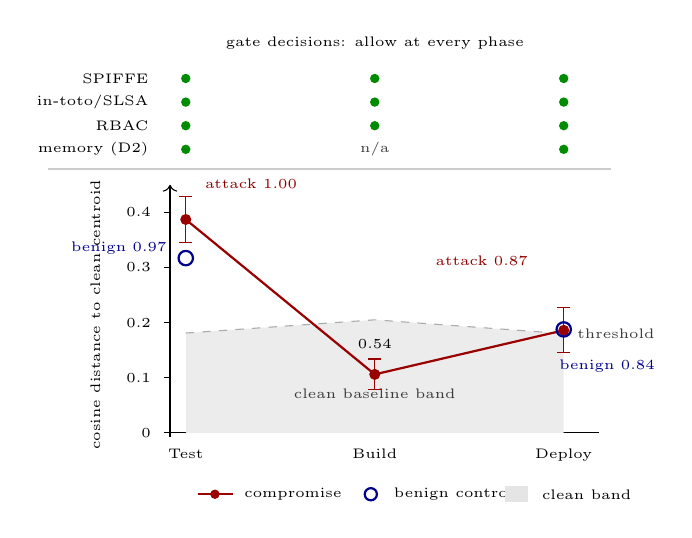
\begin{tikzpicture}[font=\scriptsize]
% ===== gate ribbon (top): every phase returns allow =====
\node[anchor=east, font=\tiny] at (-0.35,4.5) {SPIFFE};
\node[anchor=east, font=\tiny] at (-0.35,4.2) {in-toto/SLSA};
\node[anchor=east, font=\tiny] at (-0.35,3.9) {RBAC};
\node[anchor=east, font=\tiny] at (-0.35,3.6) {memory (D2)};
\foreach \x in {0,2.4,4.8}{
  \foreach \y in {4.5,4.2,3.9}{ \fill[green!55!black] (\x,\y) circle (1.7pt);}
}
\fill[green!55!black] (0,3.6) circle (1.7pt);
\fill[green!55!black] (4.8,3.6) circle (1.7pt);
\node[font=\tiny, gray!50!black] at (2.4,3.6) {n/a};
\node[font=\tiny] at (2.4,4.95) {gate decisions: allow at every phase};
\draw[gray!40] (-1.75,3.35) -- (5.4,3.35);
% ===== divergence chart (bottom) =====
% axes
\draw (-0.2,0) -- (5.25,0);
\draw[->] (-0.2,-0.05) -- (-0.2,3.15);
\foreach \v/\yy in {0/0, 0.1/0.7, 0.2/1.4, 0.3/2.1, 0.4/2.8}{
  \draw (-0.28,\yy) -- (-0.2,\yy);
  \node[anchor=east, font=\tiny] at (-0.32,\yy) {\v};
}
\node[font=\tiny, rotate=90] at (-1.15,1.5) {cosine distance to clean centroid};
% clean baseline band (per-phase 95th-pct threshold on clean runs)
\fill[gray!15] (0,0) -- (0,1.267) -- (2.4,1.435) -- (4.8,1.260) -- (4.8,0) -- cycle;
\draw[dashed, gray!65] (0,1.267) -- (2.4,1.435) -- (4.8,1.260);
\node[font=\tiny, gray!45!black] at (2.4,0.5) {clean baseline band};
\node[anchor=west, font=\tiny, gray!45!black] at (4.85,1.26) {threshold};
% compromise (attack) divergence curve, with stdev error bars
\draw[thick, red!60!black] (0,2.709) -- (2.4,0.742) -- (4.8,1.302);
\foreach \x/\yv/\e in {0/2.709/0.287, 2.4/0.742/0.196, 4.8/1.302/0.287}{
  \draw[red!60!black] (\x,\yv-\e) -- (\x,\yv+\e);
  \draw[red!60!black] (\x-0.08,\yv-\e) -- (\x+0.08,\yv-\e);
  \draw[red!60!black] (\x-0.08,\yv+\e) -- (\x+0.08,\yv+\e);
  \fill[red!60!black] (\x,\yv) circle (2pt);
}
% benign controls: drift as far as the attack at each measured phase
\draw[blue!55!black, thick] (0,2.219) circle (2.6pt);
\draw[blue!55!black, thick] (4.8,1.313) circle (2.6pt);
\node[anchor=east, font=\tiny, blue!55!black] at (-0.12,2.35) {benign 0.97};
\node[anchor=north west, font=\tiny, blue!55!black] at (4.62,1.05) {benign 0.84};
% AUC annotations (attack)
\node[anchor=south west, font=\tiny, red!55!black] at (0.12,2.98)   {attack 1.00};
\node[anchor=south, font=\tiny] at (2.4,0.95)  {0.54};
\node[anchor=south west, font=\tiny, red!55!black] at (3.05,2.00) {attack 0.87};
% phase labels
\node[anchor=north, font=\tiny] at (0,-0.08)   {Test};
\node[anchor=north, font=\tiny] at (2.4,-0.08)  {Build};
\node[anchor=north, font=\tiny] at (4.8,-0.08)  {Deploy};
% legend
\draw[thick, red!60!black] (0.15,-0.78) -- (0.6,-0.78); \fill[red!60!black] (0.37,-0.78) circle (1.7pt);
\node[anchor=west, font=\tiny] at (0.62,-0.78) {compromise};
\draw[blue!55!black, thick] (2.35,-0.78) circle (2.2pt);
\node[anchor=west, font=\tiny] at (2.52,-0.78) {benign control};
\fill[gray!20] (4.05,-0.88) rectangle (4.35,-0.68);
\node[anchor=west, font=\tiny] at (4.4,-0.78) {clean band};
\end{tikzpicture}%
}
\caption{Timeline. Pipeline phases on the x-axis; the four gates' allow decisions as marks along the top; the per-phase behavioral divergence below, with its clean-baseline band. The compromise curve (red) spikes at the tester (AUC 1.00) and rises at the deployer (AUC 0.87). The benign controls (blue) drift as far at each measured phase, a benign override at the tester (0.97) and a benign atypical target at the deployer (0.84), so the compromise and benign-anomaly points coincide and no threshold on the divergence separates malice from a benign departure. That coincidence is the paper's central result.}
\label{fig:timeline}
\end{figure}

% =====================================================================
\section{Discussion: What the Gap Requires}\label{sec:discussion}
% =====================================================================

The four gates are blind by construction, and it is worth being precise about what that does and does not say, because the easy reading is wrong. The easy reading is time-of-check to time-of-use: the gates decide once and never look again, so make them look again. That reading is old, and it has an answer, continuous verification and runtime attestation, worked out over decades. If it were the diagnosis here, this paper would be a restatement. It is not the diagnosis. The continuous-mode result rules it out: the gates re-verify at every phase and still pass, so the failure cannot be that they stopped looking. What the sensitivity and continuous results together earn is a stronger and different claim. Each gate holds a predicate over the agent's identity or the artifact's provenance or the action's membership, and every one of those predicates stays true while the agent is compromised. Identity re-checked is still valid. Provenance re-checked is still correct. Re-evaluating a true predicate returns true, at any frequency. The blind window is not a gap in time between one check and the next. It is a gap in what is checked at all: no gate in the stack carries a predicate over what the agent decides once entitled, so there is nothing about the compromise for continuous verification to catch.

Closing it needs a control of a different class, and we can state its requirements without designing it. Such a control would produce a behavioral signal, some running measure of what the agent is doing rather than who it is. It would bind that signal to the pipeline phase, since the same action means different things at test and at deploy. And it would be able to withdraw authority mid-pipeline, to revoke a right it previously granted once behavior crosses a line. Continuous verification supplies the second and third of these already: it is the machinery for re-checking and revoking on a schedule. What it does not supply is the first, a predicate over behavior worth re-checking. That absence is the whole finding, and it is why continuous verification is necessary to a fix and not itself one.

The measurement adds a fourth requirement by ruling out the obvious control. A baseline-distance drift monitor, the reflex every reviewer reaches for, cannot carry the decision on its own, and the two controls say why. At the tester the monitor separates the compromise from clean at AUC 1.00, but a benign override reproduces that at 0.97, so it fires on any applied directive. At the deployer it separates at 0.87, but a benign atypical target reproduces that at 0.84, so it fires on any unfamiliar target. Concurrent work on memory-poisoning trajectories hits the same wall from the other side: a structural recall-before-act signature that flags the attack also fires on benign memory-grounded operations, which its authors read as an attack precondition rather than a predicate over malice~\cite{forensicsig}. This does not retire the monitor. A score that ranks departures keeps its triage value, and a benign run flagged at a 5\% false-positive rate is one worth a second look rather than a false accusation. What the score cannot do is decide: at the calibration that catches the attack it also stops most benign non-routine runs, and a control that halts a pipeline that often is not one a team keeps switched on. Drift marks that a run left its routine, which a simpler override check or target allowlist marks more sharply, and it carries nothing about whether the departure is adversarial. The control the gap needs must hold the predicate the drift score lacks: at the tester, whether an applied injected directive is being followed adversarially rather than an override handled in good faith; at the deployer, whether a resolved target is adversarial rather than merely unfamiliar. Both are judgments over the semantics of the content an agent acts on rather than its distance from a baseline. That is a harder requirement than adding a behavioral monitor, and naming it precisely is what this measurement contributes. We name no mechanism, sketch no sidecar, and propose no scoring function here. The construction that satisfies these requirements is the next paper's contribution, and drawing it now would collapse the boundary this paper is written to hold.

One objection lands harder than the rest, and Section~\ref{sec:results} already hands it the ammunition: at the deploy phase a target allowlist catches the attacker endpoint outright and reads the separation more sharply than the drift score does, so for the payload demonstrated here a single deployed line closes the hole the whole gate stack left open. That result is real, and it does not rescue the gates. The allowlist bites because this payload resolves to an egress target an operator can enumerate. Swap the payload for one that names no target, a flipped test verdict, a suppressed vulnerability finding, a build flag quietly turned off, and there is nothing to list: the poison is now a value carried inside an authorized action, and the drift score stays as blind to it as before, since its distance from routine drowns in the same benign variation the two controls traced. We measured this rather than leave it as an argument. Run as a second payload class against the same clean baseline (Section~\ref{sec:results}), a flipped test verdict shipping to a standard production target scores AUC 0.67 at the deployer, crossing the 5\% line on 3 of 12 runs against the target-naming payload's 6 of 12, and its deploy input is indistinguishable from a benign deploy to that same target. There is nothing for an allowlist to enumerate and less for the drift score to read. A target allowlist and a memory-write content filter each dispatch one instance of the class. Neither reads the quantity that tells the instances apart, whether the value an authorized agent resolved is the one the pipeline intended or one an adversary planted, which is the same semantic predicate the missing control must carry. The malice sits in the provenance of the memory write, and recovering it asks what the write should have said, a judgment no allowlist over targets and no distance over reasoning holds.

The requirement is easy to state and hard to meet, and saying why is what makes it credible as an open problem. Behavior is noisy: an agent's legitimate action varies run to run, so a behavioral signal carries false positives that a static predicate never does. Baselines drift as pipelines and models change, so the reference the signal is measured against is itself moving. And a false positive at deploy does not merely log; it stalls a pipeline, and throughput is the reason teams adopted agents in the first place. A runtime behavioral control has to be right often enough that its interruptions cost less than the compromises it prevents. That trade is real, and it is why the gap has stayed open.

One boundary sizes every claim above. The negative result is established for two payload classes, one production model, and one chain exercised as $B=3$ instances. Whether it holds across agent frameworks and models is the breadth a companion study is built to measure, and marking the limit here keeps the claim no larger than the evidence under it.

% =====================================================================
\section{Related Work}\label{sec:related}
% =====================================================================

Attack demonstrations against software supply chains exist, and attack studies against LLM agents exist. Neither line measures a deployed identity-and-provenance stack failing against a phase-crossing behavioral compromise in CI/CD. We read the prior work in four families and place this paper against each. The one that matters most is continuous verification, because it is the answer a reviewer will reach for, and we address it head on.

Supply-chain and CI/CD attacks form the first. The SolarWinds build compromise showed that a trusted build system can ship a signed, malicious artifact to every downstream consumer~\cite{solarwinds}. The response lineage that followed, in-toto's signed step links and SLSA's graded integrity levels, hardened the chain of custody of the artifact~\cite{intoto,slsa}. That work targets artifact integrity: it ensures the artifact came from the declared steps. The compromise here needs no break in that chain. The steps are declared, performed, and attested correctly; the adversarial content rides through them as authorized input.

LLM-agent attacks form the second. Indirect prompt injection delivers adversarial instructions through content an agent reads rather than through its operator's prompt, and the same survey literature catalogs tool misuse, an agent driven into unintended actions through its own tool interface, as a related primitive~\cite{ipi1,ipi2}. Memory poisoning plants state that a later step consumes as legitimate, and a lifecycle survey now maps that attack surface across the write, store, and recall phases of agent memory~\cite{memsurvey,mempoison1,mempoison2,mempoison3}. Most of this work demonstrates the primitive on a single agent in a chat or task setting. The nearest concurrent work drives prompt injection through live CI/CD workflows and traces the exposure to pipeline infrastructure rather than any one model~\cite{gitinject}, an attack-side echo of our finding; it demonstrates the bypass without measuring what the deployed identity and provenance gates return to it, one-shot or continuous. What none of this work does is carry the primitive across pipeline phases, behind a stack of deployed identity and provenance gates, and measure those gates' response. We take the primitive out of the chat box and run it through the pipeline the gates were built to protect.

Continuous verification and runtime attestation form the third, and closest, family. The time-of-check to time-of-use problem is old, and the response lineage is deep: continuous authorization in Zero Trust, continuous access evaluation that revokes a session when context shifts, remote and runtime attestation that re-measures a platform's integrity on a schedule rather than at boot~\cite{contverif,attestationCoker,attestationKeylime}. What every member of this family re-verifies is a property of identity, session context, or platform integrity. The attack here breaks none of those. We tested the family's core move directly by running the gates in continuous mode, and the compromise still passes, because continuous re-verification of a valid identity and a correct provenance record returns valid and correct. The contribution is to show, with a measured continuous-mode result, that this known answer is necessary and not sufficient: it re-checks the wrong invariant, and the invariant it would need, a behavioral predicate over the agent's decisions, does not exist in the deployed stack. That is the distinction between this paper and a restatement of TOCTOU.

Behavioral and insider measurement forms the fourth. UEBA systems and insider-threat studies measure drift in human behavior against a learned baseline and alert on deviation~\cite{ueba}, and the same learned-baseline anomaly detection recurs in fraud and network-intrusion settings, where a reconstruction model scores deviation from normal activity~\cite{gahiFraud}. The instrument we use is a deliberate echo of that idea, borrowed as a measurement rather than deployed as a detector, and our controls locate the limit of the borrowing: baseline distance, UEBA's core signal, marks that an agent left its routine and cannot say whether the departure is adversarial, which is why we report it as a negative result. Concurrent work on agent memory poisoning reaches that same limit by a different route, a behavioral signature that turns out to be an attack precondition and not a maliciousness predicate~\cite{forensicsig}. What is absent from that literature is any study that instruments an autonomous agent crossing CI/CD phases and measures deployed provenance gates missing its divergence. The behavioral-measurement tradition watches humans; the provenance tradition watches artifacts. The agent falls between them, and that gap is where this paper sits.

% =====================================================================
\section{Conclusion}\label{sec:conclusion}
% =====================================================================

Four gates, three deployed and one proposed as AADS D2. One compromised agent, one deceived victim, zero detections across every run. We instrumented a running pipeline, drove a real language model through the composite chain Test/Memory~$\rightarrow$~Deploy/Delegation with all four gates enforcing, and watched every gate return allow while a poisoned deployment reached production. Then we ran the gates continuously and watched them allow it again. Identity, provenance, membership, and source class each stay true while the agent is compromised, so re-checking them, at any frequency, returns the same allow. The blindness is not a tuning failure, and it is not the old time-of-check problem either. The compromise lives outside the reach of what any of these checks can see.

The obvious fix does not hold. A reasoning-drift monitor over a clean baseline separates compromised runs from clean at both agents, the tester at AUC 1.00 and the deployer at 0.87, but two controls show the separation is anomaly and not the attack. A benign override drifts as far at the tester (0.97) and a benign atypical target as far at the deployer (0.84). The monitor flags departure from routine, which an override check or a target allowlist flags more sharply, and it carries no predicate over malice. The gates miss the compromise, and the reflexive behavioral fix cannot decide it: the drift score ranks departure and holds no predicate over malice, so at best it filters a queue for a control that does not yet exist. A control that closes this gap must read whether an agent's decision is adversarial rather than merely unusual, bind that reading to the pipeline phase, and withdraw authority mid-run. We have scoped those requirements and stopped at their edge. Building the control that meets them is the next problem.

The chain and the measurement rig ship as an artifact: the YAML descriptor, the pinned model snapshots, the record/replay store, and the offline divergence instrument, so a reader can replay the four allows and the blind window for themselves.

% =====================================================================
\bibliographystyle{IEEEtran}
\bibliography{references}

\end{document}
